\chapter[Squarefree Integers and Thorin Atoms]{Squarefree Integers and the Thorin Atoms of $\Xi$}\label{ch:squarefree}

The squarefree integers\index{squarefree integers} are a simple arithmetic sequence whose fine structure is controlled by the zeros of $\zeta$, through the doubled argument $2s$. Their generating function is
\[
D(s)=\sum_{n\ge1}\frac{\mu(n)^2}{n^s}=\frac{\zeta(s)}{\zeta(2s)},
\]
so every nontrivial zero $\rho$ of $\zeta$ becomes a pole of $D$ at $\rho/2$ (unless $\zeta(\rho/2)=0$, which RH excludes), and the critical line $\operatorname{Re} s=\frac12$ is carried to $\operatorname{Re} s=\frac14$. This chapter reads that picture through two objects of Chapters~\ref{ch:10} and~\ref{ch:10b}: the P\'olya density of $\Xi$ and the Thorin measure of $1/\Xi$. Three things come out of it. Under RH the poles of $D$ in the strip $0<\operatorname{Re}s<\frac12$ correspond to the Thorin atoms $\gamma_k^2$ through $\gamma_k^2=-(2s-\frac12)^2$; the constant $\kappa$ of the squarefree problem is a combination of two tilted means of the P\'olya law; and smoothing the squarefree count by a Gamma(2) law turns its error into a positive average of the Mertens function, with Gamma(2) the largest shape for which that holds. Section~\ref{sec:sf:computing} records how the numbers quoted are computed.

The starting point is a Math StackExchange question~\cite{mathstackexchange2016} on the asymptotics of $\sum_{n\le x}\mu(n)^2n^{-\alpha}$, especially at $\alpha=1$. Section~\ref{sec:sf:classical} answers it.

\section{The classical problem}\label{sec:sf:classical}

Let $Q(x)=\sum_{n\le x}\mu(n)^2$ and $\Delta(x)=Q(x)-6x/\pi^2$. From $\mu(n)^2=\sum_{d^2\mid n}\mu(d)$,
\begin{equation}\label{eq:sf:Qd}
Q(x)=\sum_{d\le\sqrt x}\mu(d)\Bigl\lfloor\frac{x}{d^2}\Bigr\rfloor=\frac{6}{\pi^2}x-\sum_{d\le\sqrt x}\mu(d)\Bigl\{\frac{x}{d^2}\Bigr\}+O(\sqrt x),
\end{equation}
so $\Delta(x)=O(\sqrt x)$. The terms $\mu(d)\{x/d^2\}$ will return in Section~\ref{sec:sf:gamma2}.

\subsection{Perron's formula over a number field}
For a number field $K$ with Dedekind zeta function $\zeta_K$, the ideal analogue of $D$ has Euler factor $1+N(\mathfrak{p})^{-s}=(1-N(\mathfrak{p})^{-2s})/(1-N(\mathfrak{p})^{-s})$, hence equals $\zeta_K(s)/\zeta_K(2s)$, and Perron's formula\index{Perron's formula} gives
\begin{equation}\label{eq:sf:perron}
Q_\alpha(x)=\sum_{N(\mathfrak{a})\le x}\frac{\mu^2(\mathfrak{a})}{N(\mathfrak{a})^\alpha}=\frac{1}{2\pi i}\int_{(c)}\frac{\zeta_K(s+\alpha)}{\zeta_K(2s+2\alpha)}\,x^s\,\frac{ds}{s},\qquad c>\max(0,1-\alpha),
\end{equation}
for $x$ not the norm of an ideal. The integrand has a simple pole at $s=1-\alpha$, a simple pole at $s=0$, and poles at $s=\rho/2-\alpha$ for the zeros $\rho$ of $\zeta_K$ with $\zeta_K(\rho/2)\ne0$. Let $c_K=\operatorname{Res}_{s=1}\zeta_K(s)$, and define the Euler Kronecker constant\index{Euler Kronecker constant} $\gamma_K$~\cite{ihara2006} by $\zeta_K(s)=c_K/(s-1)+c_K\gamma_K+O(s-1)$.

\begin{proposition}\label{prop:sf:classical}
For $\alpha=1$ the poles at $s=1-\alpha$ and $s=0$ merge into a double pole at $s=0$, and
\begin{equation}\label{eq:sf:alpha1K}
\sum_{N(\mathfrak{a})\le x}\frac{\mu^2(\mathfrak{a})}{N(\mathfrak{a})}=\frac{c_K}{\zeta_K(2)}\bigl(\log x+\kappa_K\bigr)+o(1),\qquad \kappa_K=\gamma_K-\frac{2\zeta_K'(2)}{\zeta_K(2)} .
\end{equation}
Over $\Q$, with $A$ the Glaisher Kinkelin constant\index{Glaisher Kinkelin constant},
\begin{equation}\label{eq:sf:final}
\sum_{n\le x}\frac{\mu(n)^2}{n}=\frac{6}{\pi^2}\bigl(\log x+\kappa\bigr)+O\bigl(x^{-1/2}\bigr),
\end{equation}
where $\kappa=24\log A-\gamma_{\mathrm E}-2\log2\pi=1.7171376511\ldots$, and for real $\alpha>\frac12$ with $\alpha\ne1$ the residues at $s=1-\alpha$ and $s=0$ give
\[
\sum_{n\le x}\frac{\mu(n)^2}{n^\alpha}=\frac{6}{\pi^2}\,\frac{x^{1-\alpha}}{1-\alpha}+\frac{\zeta(\alpha)}{\zeta(2\alpha)}+O\bigl(x^{\frac12-\alpha}\bigr).
\]
\end{proposition}

\begin{proof}
Let $Q_1(x)$, as in~\eqref{eq:sf:perron}, be the left side of~\eqref{eq:sf:alpha1K}. Summation by parts from the count of squarefree ideals, $\frac{c_K}{\zeta_K(2)}x+O(x^\theta)$ with some $\theta<1$ (from $\mu^2(\mathfrak a)=\sum_{\mathfrak d^2\mid\mathfrak a}\mu(\mathfrak d)$ and the ideal count $c_Ky+O(y^{1-1/[K:\Q]})$), gives $Q_1(x)=\frac{c_K}{\zeta_K(2)}\log x+C+O(x^{\theta-1})$. As $s\downarrow0$, $s\int_1^\infty Q_1(t)t^{-s-1}dt=\zeta_K(1+s)/\zeta_K(2+2s)$ is therefore $\frac{c_K}{\zeta_K(2)}\frac1s+C+o(1)$, and it is also $\frac{c_K}{\zeta_K(2)}(\frac1s+\kappa_K)+O(s)$, because $\kappa_K$ is the logarithmic derivative of $(s-1)\zeta_K(s)/\zeta_K(2s)$ at $s=1$. So $C=\frac{c_K}{\zeta_K(2)}\kappa_K$, and the main term is the residue at the double pole. Over $\Q$ use $\gamma_{\Q}=\gamma_{\mathrm E}$ and $\zeta'(2)/\zeta(2)=\gamma_{\mathrm E}+\log2\pi-12\log A$. For the error term, write $B(x)=\sum_{n\le x}(\mu(n)^2-6/\pi^2)=\Delta(x)+O(1)=O(\sqrt x)$ and sum by parts: the tail $\int_x^\infty B(t)t^{-2}dt$ and the boundary term $B(x)/x$ are both $O(x^{-1/2})$. For $\alpha\ne1$ the same summation by parts gives the error $O(x^{\frac12-\alpha})$ and a constant which, as a function of $\alpha$, is meromorphic in $\operatorname{Re}\alpha>\frac12$ and equals $\zeta(\alpha)/\zeta(2\alpha)$ for $\alpha>1$, hence for all $\alpha>\frac12$.
\end{proof}

The answers in~\cite{mathstackexchange2016} give the $\log x$ term and, for $\alpha\ne1$, the first main term; the second answer reaches~\eqref{eq:sf:final} with error $o(1)$ and the constant left as $\sum_n(\mu(n)^2-6/\pi^2)/n$, which equals $-2\zeta'(2)/\zeta(2)^2$. For $\frac12<\alpha<1$ the constant $\zeta(\alpha)/\zeta(2\alpha)$ is negative, for example $\zeta(\frac34)/\zeta(\frac32)=-1.3173\ldots$; Corollary~\ref{cor:sf:sign} reads the sign through the P\'olya density.

\section{The P\'olya density}\label{sec:sf:polya}

Let $\xi$, $\Xi$ and P\'olya's kernel $\Phi$ be as in~\eqref{eq:ch10polya}\index{P\'olya kernel}, so that $\xi(\frac12+z)=\int_{\R}\Phi(u)e^{zu}\,du$ for all complex $z$, and let $W_\zeta$, with density $\Phi/\Xi(0)$, be the P\'olya variable of $\zeta$ (Lemma~\ref{lem:10bkernel} and the paragraph after it). Put $T=W_\zeta/2$, whose density is $p(t)=2\Phi(2t)/\Xi(0)$, and $M_T(\theta)=\E[e^{\theta T}]$. Then
\begin{equation}\label{eq:sf:xiM}
\xi\bigl(\tfrac12+w\bigr)=\xi\bigl(\tfrac12\bigr)\,M_T(2w),\qquad \xi\bigl(\tfrac12\bigr)=0.4971207781\ldots
\end{equation}
Applying the definition of $\xi$ at $s$ and $2s$, and the duplication formula for $\Gamma(s)$, gives the following.

\begin{proposition}\label{prop:sf:polya}
For all $s$,
\[
\frac{\zeta(s)}{\zeta(2s)}=\omega(s)\,\frac{M_T(2s-1)}{M_T(4s-1)},\qquad \omega(s)=\frac{2s-1}{s-1}\,2^{s}\,\pi^{-(s+1)/2}\,\Gamma\Bigl(\frac{s+1}{2}\Bigr).
\]
\end{proposition}

The factor $1/(s-1)$ carries the pole at $s=1$, and $2s-1$ gives the zero of $D$ at $s=\frac12$, where $\zeta(2s)$ has its pole. In $\operatorname{Re}s>-1$ every other singularity of $D$ is a zero of $M_T(4s-1)$; the poles of $\Gamma(\frac{s+1}2)$ give the poles of $D$ at $s=-1,-3,\dots$.

\begin{corollary}[sign of the constant]\label{cor:sf:sign}
For real $\alpha>-1$ with $\alpha\ne\frac12,1$, the sign of $\zeta(\alpha)/\zeta(2\alpha)$ is the sign of $(2\alpha-1)/(\alpha-1)$. In particular it is negative exactly on $\frac12<\alpha<1$.
\end{corollary}

\begin{proof}
$M_T>0$ on the real line, and the gamma factor in $\omega$ is positive for $\alpha>-1$. Directly, $\zeta<0$ on $(-2,1)$ and $\zeta>0$ on $(1,\infty)$.
\end{proof}

At $\alpha=\frac34$, for instance,
\[
\omega\bigl(\tfrac34\bigr)=-1.3461\ldots,\qquad \frac{M_T(\frac12)}{M_T(2)}=\frac{\xi(\frac34)}{\xi(\frac32)}=0.9786\ldots,
\]
and their product is $\zeta(\frac34)/\zeta(\frac32)=-1.3173\ldots$.

\subsection{The constant as tilted P\'olya means}
Let $\E_\theta$ denote expectation under the tilted law $e^{\theta t}p(t)/M_T(\theta)$, so that $\E_\theta[T]=(\log M_T)'(\theta)$. Index the zeros of $\xi$ as $\rho=\frac12+i\gamma_\rho$ and let $\sum_\rho$ run over those with $\operatorname{Re}\gamma_\rho>0$, with multiplicity. By Hadamard's product and~\eqref{eq:sf:xiM},
\begin{equation}\label{eq:sf:logM}
\log M_T(\theta)=\sum_\rho\log\Bigl(1+\frac{\theta^2}{4\gamma_\rho^2}\Bigr),\qquad \E_\theta[T]=\sum_\rho\frac{2\theta}{\theta^2+4\gamma_\rho^2}.
\end{equation}

\begin{theorem}\label{thm:sf:const}
The constant in~\eqref{eq:sf:final} is
\[
\begin{aligned}
\kappa&=2+\log2-\tfrac12\log\pi-\tfrac12\gamma_{\mathrm E}+2\,\E_1[T]-4\,\E_3[T]\\
&=2+\log2-\tfrac12\log\pi-\tfrac12\gamma_{\mathrm E}+\sum_\rho\Bigl(\frac{4}{1+4\gamma_\rho^2}-\frac{24}{9+4\gamma_\rho^2}\Bigr).
\end{aligned}
\]
\end{theorem}

\begin{proof}
$\kappa$ is the logarithmic derivative of $(s-1)D(s)$ at $s=1$. Take logarithms in Proposition~\ref{prop:sf:polya}, differentiate at $s=1$, use $\psi(1)=-\gamma_{\mathrm E}$, and apply~\eqref{eq:sf:logM}.
\end{proof}

Numerically $\E_1[T]=0.0115478545$ and $\E_3[T]=0.0345331158$, and the theorem reproduces $\kappa$ to twenty digits. The first sixty zeros contribute $-0.0944$ of the zero sum $-0.1150$, the tail being about $-5\sum_{k>60}\gamma_k^{-2}$. Thus the arithmetic content of the constant is two tilted means of the P\'olya law, at the tilts $1=2s-1$ and $3=4s-1$ evaluated at $s=1$.

Comparing coefficients of $\theta^{2m}$ in~\eqref{eq:sf:logM} gives the cumulants of $W_\zeta=2T$, as in Proposition~\ref{prop:10bcumulants}:
\begin{equation}\label{eq:sf:cumulants}
\kappa_{2m}(2T)=(-1)^{m+1}\frac{(2m)!}{m}S_m,\qquad S_m=\sum_\rho\gamma_\rho^{-2m},
\end{equation}
and in particular $S_1=2\operatorname{Var}(T)=0.0231049931\ldots$ These identities are unconditional. Under RH the even cumulants of $T$ alternate in sign.

\section{Thorin atoms are the poles in the strip}\label{sec:sf:thorin}

Generalized gamma convolutions (GGC) and their Thorin measures are as in Definition~\ref{def:ch10ggc}; their Laplace transforms continue analytically and without zeros to $\C\setminus(-\infty,0]$ (Lemma~\ref{lem:ch10nonvanish}).

\begin{proposition}[Theorem~\ref{thm:10bmain} for $\zeta$; after \cite{polson2017}]\label{prop:sf:thorin}
RH holds if and only if the function $u\mapsto\xi(\frac12)/\xi(\frac12+\sqrt u)$ is a GGC Laplace transform. Then
\[
\frac{\xi(\frac12)}{\xi(\frac12+\sqrt u)}=\prod_{k\ge1}\Bigl(1+\frac{u}{\gamma_k^2}\Bigr)^{-1}=\E\bigl[e^{-uY}\bigr],\qquad Y=\sum_{k\ge1}\frac{E_k}{\gamma_k^2},
\]
with $E_k$ independent standard exponential variables, drift $0$ and Thorin measure $\tau=\sum_k\delta_{\gamma_k^2}$. Moreover $\E[Y]=2\operatorname{Var}(T)$.
\end{proposition}

\begin{proof}
This is Theorem~\ref{thm:10babstract} for $E(z)=\xi(\frac12+z)/\xi(\frac12)$, the function $\Xi_\zeta$ of Definition~\ref{def:10bxi} normalised at $0$; the mean is $S_1$, by~\eqref{eq:sf:cumulants}.
\end{proof}

Theorem~\ref{thm:10babstract} applies equally to Dedekind zeta functions (Definition~\ref{def:10bxi}). Let $\xi_K(s)=s(s-1)|d_K|^{s/2}\Gamma_{\R}(s)^{r_1}\Gamma_{\C}(s)^{r_2}\zeta_K(s)$, with $\Gamma_{\R}(s)=\pi^{-s/2}\Gamma(\frac s2)$ and $\Gamma_{\C}(s)=2(2\pi)^{-s}\Gamma(s)$.

\begin{proposition}[Theorem~\ref{thm:10babstract} for $\zeta_K$]\label{prop:sf:thorinK}
If $\zeta_K(\frac12)\ne0$, then $\xi_K(\frac12)/\xi_K(\frac12+\sqrt u)$ is a GGC Laplace transform if and only if the Riemann hypothesis holds for $\zeta_K$, and its Thorin measure is then $\sum_k\delta_{\gamma_k^2}$ over the positive ordinates of the zeros of $\zeta_K$.
\end{proposition}

A real zero $\frac12+x$ with $x>0$, a Siegel zero in particular, gives a pole at $u=x^2>0$, as in the proof of Theorem~\ref{thm:ch10general}. The hypothesis $\zeta_K(\frac12)\ne0$ fixes the normalisation: Armitage~\cite{armitage1972} exhibited a number field, from a construction of Serre, where it fails, and there one divides by $u^m$, where $2m$ is the order of the zero at $\frac12$, as in Definition~\ref{def:10bxi}.

\subsection{The recentred series}
Put $s=\frac14+\frac12\sqrt u$, so that $2s=\frac12+\sqrt u$. By Proposition~\ref{prop:sf:polya} and~\eqref{eq:sf:xiM},
\[
D\bigl(\tfrac14+\tfrac12\sqrt u\bigr)=\omega\bigl(\tfrac14+\tfrac12\sqrt u\bigr)\,\xi\bigl(\tfrac14+\tfrac12\sqrt u\bigr)\,\frac{1}{\xi(\frac12+\sqrt u)},
\]
and under RH the last factor is $\xi(\frac12)^{-1}\E[e^{-uY}]$. The atom $\gamma_k^2$ of the Thorin measure gives the pole at $u=-\gamma_k^2$, that is at $s=\frac14\pm\frac i2\gamma_k=\rho_k/2$.\index{Thorin atom} Under RH the poles of the squarefree series in $0<\operatorname{Re} s<\frac12$ are therefore exactly the Thorin atoms of $1/\Xi$, and the same holds over $K$ under the Riemann hypothesis for $\zeta_K$ by Proposition~\ref{prop:sf:thorinK}, with an extra pole at $s=\frac14$ when $\zeta_K(\frac12)=0$.

\subsection{What each atom contributes}
At a simple zero, the Perron residue of $D(s)x^s/s$ at $\rho/2$ is $R_\rho\,x^{\rho/2}$ with
\begin{equation}\label{eq:sf:Rrho}
R_\rho=\frac{\zeta(\rho/2)}{\rho\,\zeta'(\rho)},\qquad R_{\rho_1}=0.02880-0.09618\,i,\quad |R_{\rho_1}|=0.10040\ldots
\end{equation}
Formally\index{explicit formula} $\Delta(x)\approx1+2\operatorname{Re}\sum_kR_{\rho_k}x^{\rho_k/2}$, where $1$ is the residue at $s=0$. Under RH every term has size $x^{1/4}$. Figure~\ref{fig:sf:atoms} compares sixty atoms with the exact error.

\begin{figure}[t]
\centering
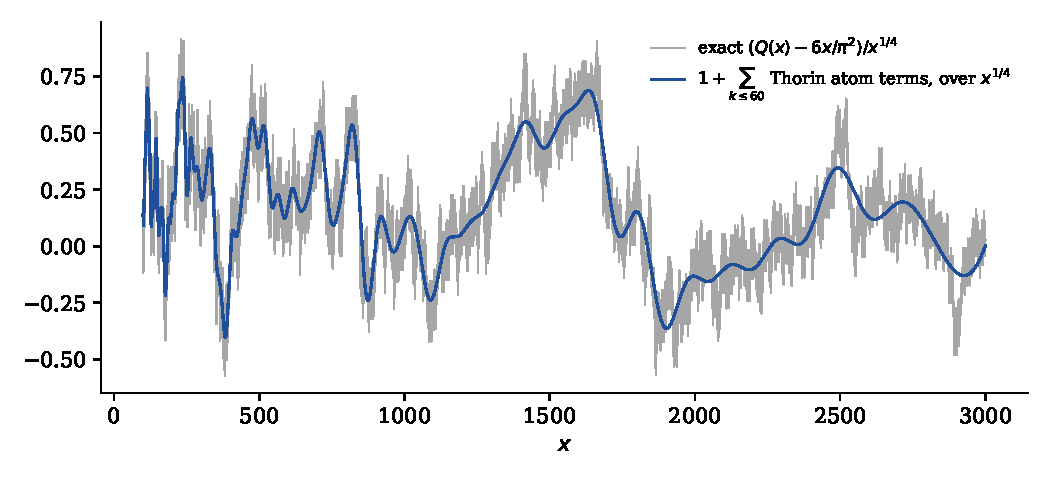
\includegraphics[width=\textwidth]{figs/sf_atoms.pdf}
\caption{The normalised error $\Delta(x)/x^{1/4}$ on $[100,3000]$ (grey) and the contribution of the first sixty Thorin atoms, $\bigl(1+2\operatorname{Re}\sum_{k\le60}R_{\rho_k}x^{\rho_k/2}\bigr)/x^{1/4}$ (blue). Correlation about $0.92$.}
\label{fig:sf:atoms}
\end{figure}

The atom series is not known to converge, even on RH: the Perron weight $1/s$ decays only like $1/|\gamma|$, and nothing controls the sizes of $\zeta(\rho/2)$ and $1/\zeta'(\rho)$ well enough. On RH, Montgomery and Vaughan~\cite{montgomeryvaughan1981} proved $\Delta(x)\ll x^{1/3+\varepsilon}$ and Liu~\cite{liu2016} $\Delta(x)\ll x^{11/35+\varepsilon}$; the conjectured bound $\Delta(x)\ll x^{1/4+\varepsilon}$ remains open on RH~\cite{mot2021,gmrr2021} (Open Problem~\ref{op:sfquarter}).

\section{Smoothed, averaged and extreme values}\label{sec:sf:smooth}

\subsection{Exponential smoothing}
Let $S(x)=\sum_n\mu(n)^2e^{-n/x}=\frac{1}{2\pi i}\int_{(2)}\Gamma(s)D(s)x^s\,ds$.

\begin{theorem}\label{thm:sf:smooth}
RH holds if and only if $S(x)=6x/\pi^2+O_\varepsilon(x^{1/4+\varepsilon})$ for every $\varepsilon>0$. Under RH with simple zeros, and with the zeros summed over $\gamma_k<T_\nu$ for a suitable sequence $T_\nu\to\infty$~\cite[Ch.~14]{titchmarsh1986},
\[
S(x)=\frac{6}{\pi^2}x+1+2\operatorname{Re}\sum_k\frac{\Gamma(\rho_k/2)\,\zeta(\rho_k/2)}{2\,\zeta'(\rho_k)}\,x^{\rho_k/2}-\frac{\zeta(-1)}{2\zeta'(-2)}\,\frac{\log x}{x}+O\Bigl(\frac1x\Bigr).
\]
\end{theorem}

\begin{proof}
Assume RH. Then $1/\zeta(\sigma+it)\ll|t|^\varepsilon$ for $\sigma\ge\frac12+\varepsilon$~\cite[Thm.~14.2]{titchmarsh1986}, $\zeta$ grows polynomially on vertical lines and $\Gamma$ decays exponentially, so the line of integration moves to $\operatorname{Re} s=\frac14+\varepsilon$, crossing only the pole at $s=1$. Moving further left collects the atoms at $\rho/2$, the residue $1$ at $s=0$, and the double pole at $s=-1$, where $\Gamma$ has a pole and $\zeta(2s)$ a trivial zero.

Conversely, the Mellin transform of $S(1/y)-6/(\pi^2y)$ on $(0,1)$ plus that of $S(1/y)$ on $(1,\infty)$ equals $\Gamma(s)D(s)-6/(\pi^2(s-1))$, and the hypothesis makes it analytic in $\operatorname{Re} s>\frac14$. Since $\Gamma$ has no zeros, $D$ is analytic there except at $s=1$. Suppose $\zeta(\rho)=0$ with $\beta=\operatorname{Re}\rho>\frac12$. Then $\rho/2$ lies in $\operatorname{Re} s>\frac14$, so its pole must cancel: $\zeta(\rho/2)=0$. By the functional equation, $\rho'=1-\overline{\rho}/2$ is a zero with $\operatorname{Re}\rho'=1-\beta/2>\frac12$ and $\operatorname{Im}\rho'=\operatorname{Im}\rho/2$. Iterating produces distinct zeros accumulating at $\frac23$, the fixed point of $\beta\mapsto1-\beta/2$; they are distinct because $\zeta$ has no real zeros in $(0,1)$. This is impossible for a function analytic and not identically zero at $\frac23$. This descent is due to Keith Conrad; Mossinghoff, Oliveira e Silva and Trudgian~\cite{mot2021} give it for the sharp count.
\end{proof}

Table~\ref{tab:sf:smooth} checks the expansion at four values of $x$.

\begin{table}[t]
\centering
\begin{tabular}{rccc}
\toprule
$x$ & $S(x)-6x/\pi^2-1$ & forty atoms & $-\frac{\zeta(-1)}{2\zeta'(-2)}\frac{\log x}{x}$\\
\midrule
$10^3$ & $-9.711\times10^{-3}$ & $\phantom{-}8.2\times10^{-5}$ & $-9.45\times10^{-3}$\\
$10^4$ & $-1.577\times10^{-3}$ & $-2.83\times10^{-4}$ & $-1.26\times10^{-3}$\\
$3\cdot10^4$ & $-7.41\times10^{-4}$ & $-2.59\times10^{-4}$ & $-4.70\times10^{-4}$\\
$10^5$ & $\phantom{-}4.23\times10^{-4}$ & $\phantom{-}5.83\times10^{-4}$ & $-1.58\times10^{-4}$\\
\bottomrule
\end{tabular}
\caption{Theorem~\ref{thm:sf:smooth}. The left column equals the sum of the other two to within $4\times10^{-5}$ for $x\ge10^4$; at $x=10^3$ the difference, $-3.4\times10^{-4}$, is the $O(1/x)$ term $-0.339/x$ of the theorem. The atoms are damped by $\Gamma(\rho/2)$, of size $e^{-\pi\gamma/4}$.}
\label{tab:sf:smooth}
\end{table}

\subsection{Mean square and extreme values}

\begin{theorem}\label{thm:sf:meansq}
RH holds if and only if $\int_X^{2X}\Delta(x)^2\,dx\ll_\varepsilon X^{3/2+\varepsilon}$ for every $\varepsilon>0$.
\end{theorem}

\begin{proof}
Let $F(s)=\int_1^\infty\Delta(x)x^{-s-1}dx=D(s)/s-6/(\pi^2(s-1))$. Under RH, $F$ is analytic in $\operatorname{Re} s>\frac14$, and the Lindel\"of bounds $\zeta(\sigma+it)\ll|t|^{1/4+\varepsilon}$ and $1/\zeta(2\sigma+2it)\ll|t|^\varepsilon$ for $\sigma\ge\frac14+\varepsilon$ give $|F(\sigma+it)|\ll|t|^{-3/4+2\varepsilon}$. The bound is uniform in $\sigma\ge c=\frac14+\varepsilon$, and $F$ is bounded near $s=1$, so $\sup_{\sigma>c}\int_{\R}|F(\sigma+it)|^2\,dt<\infty$. Since $F(s)=\int_0^\infty\Delta(e^v)e^{-sv}\,dv$ for $\operatorname{Re}s>\frac12$, the Paley Wiener theorem for the half plane $\operatorname{Re}s>c$ gives $\int_0^\infty\Delta(e^v)^2e^{-2cv}\,dv<\infty$, that is $\int_1^\infty\Delta(x)^2x^{-2c-1}dx<\infty$, and hence $\int_X^{2X}\Delta^2\ll X^{3/2+2\varepsilon}$. Conversely, Cauchy Schwarz turns the hypothesis into absolute convergence of the integral for $F$ in $\operatorname{Re} s>\frac14$, and the descent in the proof of Theorem~\ref{thm:sf:smooth} gives RH.
\end{proof}

\begin{corollary}[part (ii) after Evelyn and Linfoot~\cite{evelynlinfoot1931} and Stark~\cite{stark1966}]\label{cor:sf:omega}
(i) Under RH, $|\Delta(x)|\le X^{1/4+\varepsilon}$ for all $x\in[X,2X]$ outside a set of measure $O(X^{1-\varepsilon})$.

(ii) Unconditionally, with $|R_{\rho_1}|=0.10040\ldots$ from~\eqref{eq:sf:Rrho},
\[
\limsup_{x\to\infty}\frac{\Delta(x)}{x^{1/4}}\ge|R_{\rho_1}|,\qquad\liminf_{x\to\infty}\frac{\Delta(x)}{x^{1/4}}\le-|R_{\rho_1}| .
\]
\end{corollary}

\begin{proof}
(i) is Chebyshev's inequality. For (ii) suppose $\Delta(x)\le c\,x^{1/4}$ for $x\ge x_0$, with $c<|R_{\rho_1}|$. The function $c\,x^{1/4}-\Delta(x)$ is eventually nonnegative and its Mellin transform $c/(s-\frac14)-F(s)$ has no real singularity in $(\frac14,\infty)$, since $\zeta(2s)$ has no real zeros there. By Landau's theorem (Lemma~\ref{lem:10clandau}, \cite{landau1905})\index{Landau's lemma} the transform converges in $\operatorname{Re} s>\frac14$, which already forces RH by the descent in the proof of Theorem~\ref{thm:sf:smooth}, and at $s=\sigma+\frac i2\gamma_1$
\[
\Bigl|\frac{c}{s-\frac14}-F(s)\Bigr|\le\frac{c}{\sigma-\frac14}-F(\sigma)+O(1)=\frac{c}{\sigma-\frac14}+O(1).
\]
As $\sigma\downarrow\frac14$ the left side is at least $|R_{\rho_1}|/(\sigma-\frac14)+O(1)$, since $F$ has a pole at $\rho_1/2$ with residue $R_{\rho_1}$ if $\rho_1$ is simple and a pole of higher order otherwise. Hence $|R_{\rho_1}|\le c$, a contradiction. The lower bound is symmetric.
\end{proof}

Part (ii) is Landau's oscillation argument applied to the first zero. Evelyn and Linfoot~\cite{evelynlinfoot1931} proved $\Delta(x)=\Omega(x^{1/4})$, and Stark~\cite{stark1966} gave the first effective constant, $2(1-\gamma_1/\gamma_2)|R_{\rho_1}|=0.0657\ldots$; Landau's argument gives the larger constant of (ii), but not effectively. Using many zeros, Mossinghoff, Oliveira e Silva and Trudgian~\cite{mot2021} prove $\limsup_{x\to\infty}\Delta(x)/x^{1/4}>3$ and $\liminf_{x\to\infty}\Delta(x)/x^{1/4}<-3$, and computing $Q(x)$ for all $x\le10^{18}$ they find $|\Delta(x)|<1.12543\,x^{1/4}$ there. Sieving to $2\times10^7$ and sampling at the integers gives root mean squares of $\Delta/X^{1/4}$ on $[X,2X]$ of $0.280$, $0.255$, $0.281$ and $0.353$ for $X=10^4,\ldots,10^7$, and maxima of $|\Delta|/X^{1/4}$ between $0.68$ and $0.98$.

\subsection{How much smoothing the sharp count needs}
Let $G_{n,x}$ have the Gamma($n$) law with mean $x$. It concentrates on a window of width $x/\sqrt n$, and $\E\,Q(G_{n,x})\to Q(x)$ as $n\to\infty$ when $x$ is not a squarefree integer.

\begin{proposition}\label{prop:sf:gamman}
Under RH, uniformly in $n\ge1$,
\[
\E\,Q(G_{n,x})=\frac{6}{\pi^2}x+O_\varepsilon\bigl(x^{1/4+\varepsilon}n^{1/8+\varepsilon}\bigr).
\]
\end{proposition}

\begin{proof}
With rate $\lambda=n/x$, $\E\,Q(G)=\frac1{2\pi i}\int D(s)\frac{\Gamma(s+n)}{s\,\Gamma(n)}(x/n)^s\,ds$. Shift to $\operatorname{Re} s=c=\frac14+\varepsilon$. From $|\Gamma(n+c+it)/\Gamma(n+c)|^{-2}=\prod_{k\ge0}(1+t^2/(n+c+k)^2)$, on that line
\[
\frac{|\Gamma(n+c+it)|}{\Gamma(n)}\ll n^c\exp\bigl(-c_0\min(t^2/n,|t|)\bigr)
\]
for an absolute $c_0>0$. With $|D(c+it)|\ll|t|^{1/4+\varepsilon}$ the integral is therefore
\[
\ll x^c\int(1+|t|)^{-3/4+\varepsilon}e^{-c_0\min(t^2/n,|t|)}\,dt\ll x^cn^{1/8+\varepsilon}.
\]
\end{proof}

At $n\asymp x^2$ the window has width $O(1)$ and the bound is the trivial $x^{1/2}$. The loss $n^{1/8}$ is the growth $|t|^{1/4}$ of $\zeta$ on $\operatorname{Re} s=\frac14$ integrated against $dt/|t|$ up to $|t|\asymp\sqrt n$. Removing it needs cancellation in $\int D(\frac14+it)x^{it}dt/t$, not a bound on its size.


\section{Gamma(2) smoothing and the Mertens function}\label{sec:sf:gamma2}

Return to the terms $\mu(d)\{x/d^2\}$ of \eqref{eq:sf:Qd}. Steutel and Thiemann \cite{steutelthiemann1989} studied when the integer and fractional parts of a random variable are independent, the exponential law being the basic case. We randomise $x$ by a Gamma(2) law and compute every term in closed form.

\subsection{Expected fractional parts}
Let $G$ have the Gamma(2) density $\lambda^2te^{-\lambda t}$ and $\theta=\lambda a$. Since $P(G\ge ma)=(1+m\theta)e^{-m\theta}$,
\begin{equation}\label{eq:sf:g}
\begin{aligned}
\E\lfloor G/a\rfloor&=\frac{1}{e^\theta-1}+\frac{\theta}{4\sinh^2(\theta/2)},\\
\E\{G/a\}=g(\theta)&=\frac2\theta-\frac{1}{e^\theta-1}-\frac{\theta}{4\sinh^2(\theta/2)} .
\end{aligned}
\end{equation}
With $\theta=2y$ the term $\theta/(4\sinh^2(\theta/2))$ equals $\theta^{-1}(y/\sinh y)^2$, and $(y/\sinh y)^2$ is the Laplace transform at $y^2/2$ of the sum of two independent hitting times of $1$ by a three dimensional Bessel process, through which Williams represents $\xi$ (Section~\ref{sec:ch10bpy}; \cite[Section~5]{williams1990} and \cite[(6) to (8) and Table~2]{bpy2001}). Expanding $1/(e^\theta-1)=\sum_me^{-m\theta}$ gives the Mellin transform $\int_0^\infty g(\theta)\theta^{s-1}d\theta=-(1+s)\Gamma(s)\zeta(s)$ for $0<\operatorname{Re} s<1$. Take $\lambda=2/X$, so that $\E G=X$, and write $G_X$. Summing \eqref{eq:sf:g} over $a=d^2$, now over all $d$ since $0\le g(\theta)\le\min(1,2/\theta)$,
\begin{equation}\label{eq:sf:EQ}
\E\,Q(G_X)=\sum_{n\ge1}\mu(n)^2\Bigl(1+\frac{2n}{X}\Bigr)e^{-2n/X}=\frac{6}{\pi^2}X-\sum_{d\ge1}\mu(d)\,g\Bigl(\frac{2d^2}{X}\Bigr).
\end{equation}
Table~\ref{tab:sf:EQ} checks this identity numerically.

\subsection{The Mertens representation}

\begin{theorem}\label{thm:sf:mertens}
The function
\[
f_V(v)=-2g'(v)=\frac{4}{v^2}-\frac{v\cosh(v/2)}{2\sinh^3(v/2)},\qquad v>0,
\]
is a probability density with $P(V\ge v)=2g(v)$ and $\E[V^s]=-2\Gamma(s+2)\zeta(s)$ for $0<\operatorname{Re} s<1$. With $M(t)=\sum_{d\le t}\mu(d)$ the Mertens function,
\[
\E\,Q(G_X)=\frac{6}{\pi^2}X-\frac12\,\E\Bigl[M\Bigl(\sqrt{XV/2}\Bigr)\Bigr].
\]
Moreover $f_V$ is twice the difference between the continuous and the integer rate mixtures of Gamma(2) densities $\gamma_{2,\lambda}(v)=\lambda^2ve^{-\lambda v}$:
\[
f_V(v)=2\Bigl(\int_0^\infty\gamma_{2,\lambda}(v)\,d\lambda-\sum_{m\ge1}\gamma_{2,m}(v)\Bigr).
\]
\end{theorem}

\begin{proof}
With $x=v/2$, $f_V\ge0$ reads $(\sinh x/x)^3\ge\cosh x$, which is Lazarevi\'c's inequality \cite{lazarevic1966}. The mass is $2g(0+)=1$. The moments follow by parts from the Mellin transform of $g$. Since $P(\sqrt{XV/2}\ge d)=2g(2d^2/X)$, the expectation of $M$ is $2\sum_d\mu(d)g(2d^2/X)$, which is \eqref{eq:sf:EQ}. Finally $\int_0^\infty\gamma_{2,\lambda}(v)d\lambda=2/v^2$ and $\sum_m\gamma_{2,m}(v)=v\cosh(v/2)/(4\sinh^3(v/2))$.
\end{proof}

After Gamma(2) smoothing, the squarefree error is exactly minus half the mean of the Mertens function at a random point, and the randomising law is itself the gap between a continuous and a lattice mixture of Gamma(2) laws. With exponential smoothing the same holds with $f_{V_1}(v)=2/v^2-1/(2\sinh^2(v/2))$, positive since $\sinh x\ge x$, and $S(x)=6x/\pi^2-\frac12\E M(\sqrt{xV_1})$.

\begin{corollary}\label{cor:sf:mertens}
(i) Unconditionally $\E\,Q(G_X)=6X/\pi^2+o(X^{1/2})$. (ii) RH holds if and only if $\E\,Q(G_X)=6X/\pi^2+O_\varepsilon(X^{1/4+\varepsilon})$ for every $\varepsilon>0$. (iii) Under RH with simple zeros, and with the zeros summed over $\gamma_k<T_\nu$ for a suitable sequence $T_\nu\to\infty$ \cite[Ch.~14]{titchmarsh1986},
\[
\begin{aligned}
\E\,Q(G_X)={}&\frac{6}{\pi^2}X+1+2\operatorname{Re}\sum_k\Bigl(1+\frac{\rho_k}2\Bigr)\frac{\Gamma(\rho_k/2)\,\zeta(\rho_k/2)}{2\,\zeta'(\rho_k)}\Bigl(\frac X2\Bigr)^{\rho_k/2}\\
&-\frac{\pi^2}{3\zeta(3)\,X}+O\Bigl(\frac1{X^2}\Bigr).
\end{aligned}
\]
\end{corollary}

\begin{proof}
By Littlewood's criterion \cite[Ch.~14]{titchmarsh1986}, RH is equivalent to $M(t)\ll t^{1/2+\varepsilon}$, which gives (ii) forwards since $\E V^\beta<\infty$ for $\beta<1$; $M(t)=o(t)$ and dominated convergence give (i). The converse of (ii) is the descent argument of Theorem \ref{thm:sf:smooth} with kernel $(1+s)\Gamma(s)2^{-s}$, which has no zeros in $\operatorname{Re} s>0$. For (iii), shift the contour in $\frac1{2\pi i}\int(1+s)\Gamma(s)D(s)(X/2)^s\,ds$ to the left along the heights $T_\nu$. The pole at $s=-1$ is simple, since $(1+s)\Gamma(s)$ is regular there, and its residue is $-\zeta(-1)/(\zeta'(-2)X)=-\pi^2/(3\zeta(3)X)$.
\end{proof}

\begin{table}[t]
\centering
\begin{tabular}{rccc}
\toprule
$X$ & $E_X$ & $-\sum_{d\le2\cdot10^5}\mu(d)g(2d^2/X)$ & $(E_X-1)/X^{1/4}$\\
\midrule
$10^3$ & $0.9971612$ & $0.9971610$ & $-5.0\times10^{-4}$\\
$10^4$ & $1.0009452$ & $1.0009431$ & $\phantom{-}9.5\times10^{-5}$\\
$10^5$ & $0.9966202$ & $0.9965983$ & $-1.9\times10^{-4}$\\
$10^6$ & $1.0061029$ & $1.0058842$ & $\phantom{-}1.9\times10^{-4}$\\
\bottomrule
\end{tabular}
\caption{Identity \eqref{eq:sf:EQ}, with $E_X=\E Q(G_X)-6X/\pi^2$ from a sieve to $4\times10^7$. The discrepancies are the truncation of the $d$ sum. The last column divides the part of Corollary~\ref{cor:sf:mertens}(iii) beyond the constant $1$ by $X^{1/4}$; at $X=10^3$ it is mostly the term $-\pi^2/(3\zeta(3)X)$.}
\label{tab:sf:EQ}
\end{table}

\subsection{Which Gamma shapes work}
For Gamma($\nu$) smoothing the expected fractional part is
\[
g_\nu(\theta)=\frac\nu\theta-\sum_{m\ge1}\frac{\Gamma(\nu,m\theta)}{\Gamma(\nu)},
\]
and the argument above gives
\[
\E\,Q(G)=\frac{6}{\pi^2}\E G-\frac12\int_0^\infty M\bigl(\sqrt{v/\lambda}\bigr)f_{V_\nu}(v)\,dv,\qquad f_{V_\nu}=-2g_\nu',
\]
with moments
\[
\int_0^\infty v^sf_{V_\nu}(v)\,dv=-\frac{2\,\Gamma(s+\nu)\,\zeta(s)}{\Gamma(\nu)} .
\]
The poles of the Mellin transform at $s=-\nu-k$ give
\[
g_\nu(\theta)=\frac12+\frac{\zeta(-\nu)}{\Gamma(\nu+1)}\,\theta^\nu+O(\theta^{\nu+1}),
\]
so $f_{V_\nu}(v)=O(v^{\nu-1})$ at $0$ and the moment formula holds on $-\nu<\operatorname{Re} s<1$ by continuation. Is $f_{V_\nu}$ a probability density, so that the error is a positive average of $M$? The answer is a sharp threshold.

\begin{lemma}\label{lem:sf:riemann}
$f_{V_\nu}(\theta)=2\nu\bigl(1-R_\nu(\theta)\bigr)/\theta^2$, where $R_\nu(h)=h\sum_{m\ge1}\gamma_{\nu+1}(mh)$ is the right Riemann sum with step $h$ of the Gamma($\nu+1$,1) density $\gamma_{\nu+1}$. Thus $f_{V_\nu}\ge0$ if and only if $R_\nu\le1$.
\end{lemma}

\begin{proof}
Differentiate $g_\nu$ term by term, using $y\,\gamma_\nu(y)=\nu\,\gamma_{\nu+1}(y)$.
\end{proof}

For example
\[
R_1(h)=\frac{(h/2)^2}{\sinh^2(h/2)},\qquad R_2(h)=\frac{(h/2)^3\cosh(h/2)}{\sinh^3(h/2)} .
\]

\begin{theorem}\label{thm:sf:threshold}
$f_{V_\nu}\ge0$ if and only if $0<\nu\le2$.
\end{theorem}

\begin{proof}
Necessity. For $\nu>2$ the moment formula holds on $(-\nu,1)$, where $\Gamma(s+\nu)>0$. But $\zeta>0$ on $(-4,-2)$, which meets $(-\nu,1)$, so $\int v^sf_{V_\nu}dv<0$ for some real $s$ and $f_{V_\nu}$ takes negative values.

Sufficiency. The cases $\nu=1,2$ are $\sinh x\ge x$ and Theorem \ref{thm:sf:mertens}. Let $\nu=k+\eta$ with $k\in\{0,1\}$ and $0<\eta<1$, and set $R_0(x)=x/(e^x-1)$. The identity $y^\eta=\frac{\eta}{\Gamma(1-\eta)}\int_0^\infty(1-e^{-sy})s^{-\eta-1}ds$, the L\'evy Khintchine form of the Bernstein function $y^\eta$, applied to the sum and the integral defining $R_\nu(h)-1$, gives with $c=1+s$
\[
\Gamma(\nu+1)\bigl(R_\nu(h)-1\bigr)=\frac{\eta\,k!}{\Gamma(1-\eta)}\int_0^\infty s^{-\eta-1}\Bigl[\frac{1-R_k(hc)}{c^{k+1}}-\bigl(1-R_k(h)\bigr)\Bigr]ds .
\]
The bracket is nonpositive for every $c>1$ as soon as $x\mapsto(1-R_k(x))/x^{k+1}$ is nonincreasing. For $k=0$ this function is $g_1$, decreasing by the case $\nu=1$. For $k=1$ it is $\frac12f_{V_1}(x)=x^{-2}-\frac14\sinh^{-2}(x/2)$. Its derivative, with $u=x/2$, is $\frac14(\cosh u/\sinh^3u-u^{-3})$, nonpositive by Lazarevi\'c's inequality.
\end{proof}

The proof is a ladder: positivity on $(k,k+1)$ follows from monotonicity of $(1-R_k(x))/x^{k+1}$, which is $g_1$ for $k=0$ and $x^{1-k}f_{V_k}(x)/(2k)$ for $k\ge1$. It stops after two rungs because $x^{-1}f_{V_2}(x)\sim x/60$ increases near $0$, which is the statement $\zeta(-3)>0$ with $\zeta(-2)=0$. The substitution $x=v/2$ of the proof of Theorem~\ref{thm:sf:mertens} turns $f_{V_2}(v)=v^2/60+O(v^4)$ into $(\sinh x/x)^3-\cosh x=x^4/15+O(x^6)$, and $3$ is the smallest exponent for which Lazarevi\'c's inequality holds near $0$.

\section{Off the critical line}\label{sec:sf:strip}

For $\sigma\ge\frac12$ put
\[
\varphi_\sigma(u)=\frac{\xi(\sigma)}{\xi(\sigma+\sqrt u)},\qquad u\in\mathbb C\setminus(-\infty,0],
\]
with the principal root, so that $\sigma+\sqrt u$ ranges over $\operatorname{Re} s>\sigma$. For $\sigma>\frac12$ the function $\xi(\sigma+w)$ is not even in $w$, and the factors of its Hadamard product are no longer of the form $1+u/r$ with $r>0$. The Thorin structure nevertheless survives: atoms are smeared into Cauchy profiles.

By Theorem~\ref{thm:10dshift} with $a=\sigma-\frac12$, which for $\xi$ is Theorem~18 with Remark~21 of \cite{polson2018vdp}, $\varphi_\sigma$ is a GGC Laplace transform if and only if $\sigma\ge\beta^*$, where $\beta^*=\sup\{\operatorname{Re}\rho:\zeta(\rho)=0,\ 0<\operatorname{Re}\rho<1\}$; the case $\sigma=\beta^*$ follows by closure under limits. For $\sigma>\beta^*$ the Thorin measure $\tau_\sigma$ of $\varphi_\sigma$ has the density $V_{\sigma-1/2}(r)$ of that theorem, which in the variable $t=\sqrt r$ reads
\begin{equation}\label{eq:sf:closed}
\frac1\pi\,\operatorname{Re}\frac{\xi'}{\xi}(\sigma+it)\,dt,\qquad \frac{\xi'}{\xi}(s)=\frac1s+\frac1{s-1}-\frac12\log\pi+\frac12\psi\Bigl(\frac s2\Bigr)+\frac{\zeta'}{\zeta}(s),
\end{equation}
so it can be computed from $\zeta'/\zeta$ alone. A pair of zeros $\beta\pm it_\rho$ with $\delta=\sigma-\beta>0$ and $c=\delta^2+t_\rho^2$ contributes the factor $c/(c+B(u))$, with $B(u)=u+2\delta\sqrt u$, to $\varphi_\sigma$, and the density
\[
h^{(\delta)}_c(r)=\frac{\delta}{\pi}\,\frac{r+c}{\sqrt r\,\bigl((c-r)^2+4\delta^2r\bigr)}
\]
to $\tau_\sigma$. This is the density of one pair of zeros in the proof of Theorem~\ref{thm:10dshift}, since $2t\,h^{(\delta)}_c(t^2)$ is the sum of the Poisson kernels $\frac1\pi\delta/(\delta^2+(t\mp t_\rho)^2)$. Each $h^{(\delta)}_c$ is a probability density, close to a Cauchy density at $c$ of half width $2\delta\sqrt c$, and it tends to the unit mass at $c$, an atom of the Thorin measure of Proposition~\ref{prop:sf:thorin}, as $\delta\downarrow0$.

\begin{corollary}[subordination]\label{cor:sf:sub}
For $\sigma\ge\beta^*$, $\varphi_\sigma(u)=\E[e^{-uY_\sigma}]$ with
\[
Y_\sigma=\sum_{\rho=\beta+it_\rho,\ t_\rho>0}\Bigl(\frac{E_\rho}{c_\rho}+T_\rho\Bigr),\qquad c_\rho=(\sigma-\beta)^2+t_\rho^2,
\]
where the zeros are counted with multiplicity, the $E_\rho$ are independent standard exponentials and, given $E_\rho$, $T_\rho$ is the first passage time of an independent standard Brownian motion to the level $\sqrt2(\sigma-\beta)E_\rho/c_\rho$.
\end{corollary}

\begin{proof}
With $\delta=\sigma-\beta$, $c_\rho/(c_\rho+B(u))=\E\exp(-B(u)E_\rho/c_\rho)$, and $e^{-yB(u)}=e^{-yu}e^{-a\sqrt{2u}}$ with $a=\sqrt2\delta y$ is the transform of $y$ plus the passage time to the level $a$.
\end{proof}

The factor $e^{-a\sqrt{2u}}$ is the transform of the positive $\frac12$ stable law, as in the first step of Lemma~\ref{lem:10dsin2} \cite{roynetteyor2005}. Moving off the line therefore runs each exponential of Proposition \ref{prop:sf:thorin} through its own Brownian clock. Since passage times have infinite mean, $\E Y_\sigma=\infty$ for $\sigma>\frac12$, which matches the $\sqrt u$ branch point of $\varphi_\sigma$ at $0$.

Positivity of $\operatorname{Re}\xi'/\xi$ on the half plane $\operatorname{Re}s>\frac12$ is equivalent to RH by the criterion of Hinkkanen \cite{hinkkanen1997} and Lagarias \cite{lagarias1999}, and Theorem~\ref{thm:10dshift}(iv) is its Thorin form; more generally, positivity on $\operatorname{Re}s>\sigma$ is equivalent to $\sigma\ge\beta^*$ (\cite{lagarias1999}, Theorem~1.1), that is to the GGC property at $\sigma$. At $\sigma=0.65$, $t=20$ the closed form \eqref{eq:sf:closed} gives $\operatorname{Re}\xi'/\xi=0.15849$, a density of $0.05045$, and the first $300$ zero pairs give $0.15801$, the difference being the tail. A negative value of $\operatorname{Re}\xi'/\xi$ on the line $\operatorname{Re}s=\sigma$, computed with a rigorous error bound, proves a zero with real part above $\sigma$; a positive value on one line proves nothing.

\begin{figure}[t]
\centering
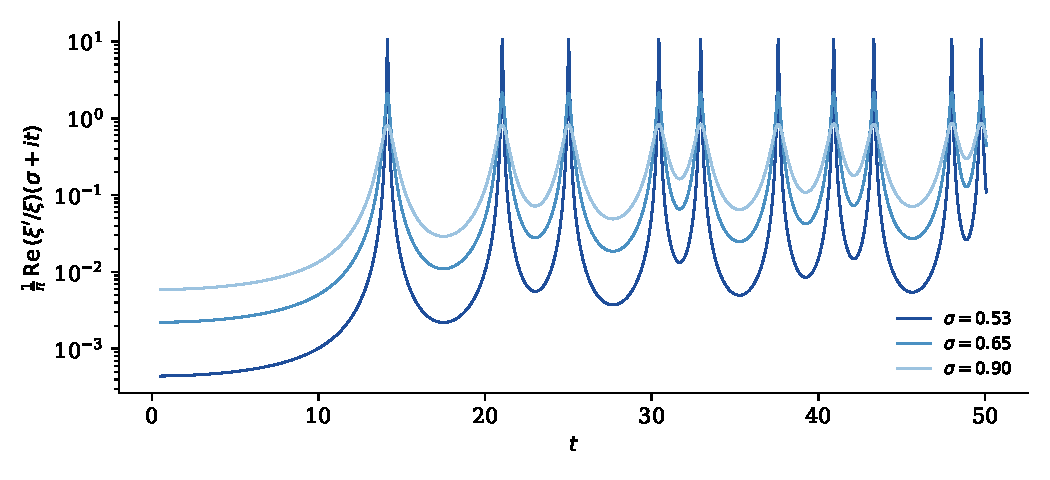
\includegraphics[width=\textwidth]{figs/sf_thorin_strip.pdf}
\caption{The function $\frac1\pi\operatorname{Re}(\xi'/\xi)(\sigma+it)$ of \eqref{eq:sf:closed}, computed from $\zeta'/\zeta$ alone, for $\sigma=0.53,0.65,0.90$ and $0.5\le t\le50$, on a logarithmic vertical scale. Under RH it is the density of $\tau_\sigma$ in the variable $t$, and each zero contributes a Cauchy profile of half width $\sigma-\frac12$ centred at its ordinate, which sharpens into an atom as $\sigma\downarrow\frac12$. The minima on $[0.5,50]$, all at $t=0.5$, are $4.4\times10^{-4}$, $2.2\times10^{-3}$ and $5.9\times10^{-3}$.}
\label{fig:sf:strip}
\end{figure}

\section{Number fields}\label{sec:sf:fields}

\subsection{The constant over $K$}
Theorem \ref{thm:sf:const} extends to every number field, which completes \eqref{eq:sf:alpha1K}.

\begin{theorem}\label{thm:sf:constK}
With the zeros of $\zeta_K$ in the critical strip written $\frac12+i\gamma_\rho$ and summed over all of them with multiplicity,
\[
\kappa_K=A_K+\sum_\rho\Bigl(\frac{2}{1+4\gamma_\rho^2}-\frac{12}{9+4\gamma_\rho^2}\Bigr),
\]
\[
A_K=2+\tfrac12\log|d_K|+r_1\bigl(\log2-\tfrac12\log\pi-\tfrac12\gamma_{\mathrm E}\bigr)+r_2\bigl(2-\gamma_{\mathrm E}-\log2\pi\bigr).
\]
\end{theorem}

\begin{proof}
From the definition of $\xi_K$,
\[
(s-1)\frac{\zeta_K(s)}{\zeta_K(2s)}=2(2s-1)\,|d_K|^{s/2}\,\frac{\Gamma_{\mathbb R}(2s)^{r_1}\Gamma_{\mathbb C}(2s)^{r_2}}{\Gamma_{\mathbb R}(s)^{r_1}\Gamma_{\mathbb C}(s)^{r_2}}\cdot\frac{\xi_K(s)}{\xi_K(2s)} .
\]
The logarithmic derivative of the elementary factor at $s=1$ is $A_K$, using $\psi(1)=-\gamma_{\mathrm E}$, $\psi(\frac12)=-\gamma_{\mathrm E}-2\log2$ and $\psi(2)=1-\gamma_{\mathrm E}$. For the rest, $\frac{\xi_K'}{\xi_K}(\frac12+w)=\sum_\rho\frac{w}{w^2+\gamma_\rho^2}$ over all zeros, taken at $w=\frac12$ minus twice its value at $w=\frac32$.
\end{proof}

For $K=\mathbb Q$ this is Theorem~\ref{thm:sf:const}, whose sum runs over $\operatorname{Re}\gamma_\rho>0$ with doubled weights. For $K=\mathbb Q(i)$, where $\zeta_K=\zeta\cdot L(s,\chi_{-4})$, both sides of the theorem give $\kappa_{\mathbb Q(i)}=1.7846166671\ldots$ to twenty digits when the zero sum is evaluated as $\frac{\xi_K'}{\xi_K}(1)-2\frac{\xi_K'}{\xi_K}(2)$; summed over the zeros below height $1000$, with a tail estimate, it agrees to six digits. The zeros of $\zeta$ and of $L(s,\chi_{-4})$ simply pool their Thorin atoms.

\subsection{A P\'olya kernel for imaginary quadratic fields}
Let $K$ be imaginary quadratic of discriminant $d$, let $a_n=\sum_{m\mid n}\chi_d(m)$ count ideals of norm $n$, and put $\lambda_n=2\pi n/\sqrt{|d|}$ and $F(k)=k(k-2)e^{-k}$. Write $\Lambda_K(s)=(\sqrt{|d|}/2\pi)^s\Gamma(s)\zeta_K(s)$, so that $\xi_K(s)=2s(s-1)\Lambda_K(s)$.

\begin{theorem}\label{thm:sf:kernel}
Let $H_K(x)=\sum_{n\ge1}a_nF(\lambda_nx)$ and $\Phi_K(v)=e^{v/2}H_K(e^v)$. Then $\Phi_K$ is even, decays doubly exponentially, and $\xi_K(\frac12+iz)=2\int_{\mathbb R}\Phi_K(v)e^{izv}dv$. If $|d|<\pi^2$, that is $d\in\{-3,-4,-7,-8\}$, then $\Phi_K>0$; consequently $\xi_K(\frac12+w)/\xi_K(\frac12)$ is the moment generating function of a probability density, and $\zeta_K(\frac12)<0$.
\end{theorem}

\begin{proof}
With $\psi_K(x)=\sum_na_ne^{-\lambda_nx}$ one has $\Lambda_K(s)=\int_0^\infty\psi_K(x)x^{s-1}dx$ and $H_K=(x^2\psi_K')'$, so two integrations by parts give $\int_0^\infty H_K(x)x^{s-1}dx=s(s-1)\Lambda_K(s)=\frac12\xi_K(s)$. Substitute $x=e^v$; the functional equation $\Lambda_K(s)=\Lambda_K(1-s)$ makes $\Phi_K$ even. Every term of $H_K$ is positive for $x>2/\lambda_1=\sqrt{|d|}/\pi$, which covers $x\ge1$ when $|d|<\pi^2$, and evenness covers the rest. Finally $\xi_K(\frac12)=-\frac12\Lambda_K(\frac12)=2\int\Phi_K>0$.
\end{proof}

The sign of $\zeta_K(\frac12)=\zeta(\frac12)L(\frac12,\chi_d)$ is known far beyond these four fields: $L(s,\chi_d)$ has no positive real zero for $-3\cdot10^8\le d<0$ \cite{watkins2004}. For $d=-4$ the Fourier identity holds to sixteen digits at $z=0$ and $z=2.5$. Beyond $|d|<\pi^2$ positivity is arithmetic. Replacing $a_n$ by its mean $L(1,\chi_d)$ makes $H_K(1)$ small, about $L(1,\chi_d)\lambda_1/6$, since $\int_0^\infty F=0$; the sign is decided by how the smallest ideal norms deviate from their average.

\begin{theorem}\label{thm:sf:inert}
If $2$ and $3$ are both inert in $K$, then $\Phi_K$ takes negative values. This holds for infinitely many fields, among them $d=-19,-43,-67,-163$.
\end{theorem}

\begin{proof}
Write $x=y\sqrt{|d|}/2\pi$, so $H_K=\sum_na_nF(ny)$. The ideal counts are multiplicative with $a_{p^e}\le e+1$, and when $2,3$ are inert $a_{2^e}$ and $a_{3^e}$ vanish for odd $e$ and equal $1$ for even $e$. Hence $a_n\le a_n^*$, where $a_n^*=0$ unless $v_2(n)$ and $v_3(n)$ are even, in which case $a_n^*$ is the number of divisors of $n2^{-v_2(n)}3^{-v_3(n)}$; in particular $a_2=a_3=0$. At $y=1.42$, $F(ny)>0$ for $n\ge2$, and
\[
H_K\le F(1.42)+\sum_{n\ge4}a_n^*F(1.42\,n)=-0.19908+0.13918<0,
\]
the sum computed to $n=4000$ with negligible tail. Finally $2$ and $3$ are both inert exactly when $d\equiv5\bmod24$, which holds for infinitely many fundamental discriminants.
\end{proof}

Since $\xi_K$ is a constant multiple of $\xi(s)\Lambda(s,\chi_d)$ (proof of Theorem~\ref{beta:thm:realchar}), $\Phi_K$ is a positive multiple of the convolution of P\'olya's kernel with the theta kernel $v\mapsto e^{3v/2}\vartheta_{\chi_d}(e^{2v})$ of Section~\ref{sec:hitexit}. So for $d=-4$ positivity also follows from Proposition~\ref{beta:prop:kernel}, and when $2$ and $3$ are inert the theta function of $\chi_d$ takes negative values (compare Section~\ref{sec:hitexit}).

All $6079$ fundamental discriminants with $|d|\le20000$ were scanned on a grid of $200$ points (Section~\ref{sec:sf:computing}); $2738$ are positive at every grid point, and a grid ten times finer changes none. Table \ref{tab:sf:kernel} sorts them by the behaviour of $2$ and $3$: the more small primes split, the more ideals of small norm, and the likelier positivity. Positivity is not decided at the centre: only $1904$ of the $3341$ failures have $\Phi_K(0)<0$. The number of positive fields per block of $2000$ discriminants falls from $337$ to between $253$ and $272$ in the last five blocks.

\begin{table}[t]
\centering
\begin{tabular}{lccc}
\toprule
& $\chi_d(3)=1$ & $\chi_d(3)=0$ & $\chi_d(3)=-1$\\
\midrule
$\chi_d(2)=1$ & $676/767$ & $334/507$ & $412/757$\\
$\chi_d(2)=0$ & $489/753$ & $178/514$ & $131/757$\\
$\chi_d(2)=-1$ & $397/761$ & $121/500$ & $0/763$\\
\bottomrule
\end{tabular}
\caption{Fields with $\Phi_K>0$ at every point of the grid of Section~\ref{sec:sf:computing}, among fundamental discriminants $-20000\le d<0$. The empty cell is Theorem \ref{thm:sf:inert}.}
\label{tab:sf:kernel}
\end{table}

\section{Computing the quantities in this chapter}\label{sec:sf:computing}

The sieve and the ideal counts are exact integer computations, done with \texttt{numpy}. The analytic quantities are floating point, computed with \texttt{mpmath} at twenty digits or more unless stated otherwise, and carry no rigorous error bounds.

\begin{itemize}
\item Squarefree indicators to $N$: start from an array of ones and zero out multiples of $d^2$ for $d\le\sqrt N$; cumulative sums give $Q$ exactly, and $\Delta$ in floating point. A sieve to $4\times10^7$ runs in seconds.
\item Tilted P\'olya means: $\E_\theta[T]=\frac12(\xi'/\xi)(\frac12+\frac\theta2)$ by numerical differentiation of $\log\xi$; no quadrature of $\Phi$ is needed. The P\'olya integral itself converges with forty terms of $\Phi$ on $[0,4]$.
\item Atom coefficients $R_\rho$: \texttt{zetazero(k)} and \texttt{diff(zeta,rho)}. Sixty zeros take under a minute.
\item Kernel signs $\Phi_K$: Kronecker symbols by quadratic reciprocity and $a_n$ by a divisor sieve to $12\sqrt{|d|}+50$, both exact; $H_K$ in floating point on $200$ points of $[1,\max(1,\sqrt{|d|}/\pi)]$. This covers $v\ge0$, evenness covers $v<0$, and beyond $\sqrt{|d|}/\pi$ every term is positive.
\item The Thorin density of Figure \ref{fig:sf:strip}: the closed form \eqref{eq:sf:closed}, on a grid refined near the first ten ordinates.
\end{itemize}

\section{The Euler product as a law}\label{sec:sf:euler}

For $\sigma>1$, $P(N=n)=\mu(n)^2n^{-\sigma}/D(\sigma)$ is a law on squarefree integers with $\log N=\sum_pB_p\log p$ for independent Bernoulli variables of success probability $p^{-\sigma}/(1+p^{-\sigma})$. As for the Euler products of Chapter~\ref{ch:09}, $\log\E N^{-w}=\log D(\sigma+w)-\log D(\sigma)$ has a L\'evy Khintchine form, here with the signed L\'evy measure $\sum_p\sum_k(-1)^{k+1}k^{-1}p^{-k\sigma}\delta_{k\log p}$ (compare \eqref{eq:ch09signed}), so by uniqueness the law of $\log N$ is not infinitely divisible; it is quasi infinitely divisible in the sense of \cite{lindnerpansato2018}. The negative part sits at even $k$ and contributes
\[
-\sum_p\sum_{j\ge1}\frac{p^{-2js}}{2j}=-\frac12\log\zeta(2s)
\]
to $\log D(s)$, the factor $\zeta(2s)^{-1/2}$: in $D(s)=\zeta(s)/\zeta(2s)$ the even $k$ carry $+1/k$ from $\zeta(s)$ and $-2/k$ from $1/\zeta(2s)$. The factor $1/\zeta(2s)$, which makes the arithmetic side signed, becomes after the change of variable $u=(2s-\frac12)^2$ the positive Thorin measure of Proposition \ref{prop:sf:thorin} on the analytic side, provided RH holds.

\subsection{Open problems}

\begin{problem}[The exponent one quarter]\label{op:sfquarter}
Prove that $\Delta(x)\ll x^{1/4+\varepsilon}$ on RH; the best exponent known on RH is $\frac{11}{35}$ (end of Section~\ref{sec:sf:thorin}). By Proposition~\ref{prop:sf:gamman} it would follow from removing the factor $n^{1/8}$ at $n\asymp x^2$, and by Corollary~\ref{cor:sf:omega} it amounts to emptying the exceptional set.
\end{problem}

\begin{problem}[How often is $\Phi_K$ positive?]\label{op:sfdensity}
Does the set of negative fundamental discriminants $d$ with $\Phi_K>0$ have positive lower density? Is there a finite set of splitting conditions on small primes under which $\Phi_K>0$ for every $d$ that satisfies them, a positive counterpart of Theorem~\ref{thm:sf:inert}?
\end{problem}

\section{Notes}

The question and both answers are in \cite{mathstackexchange2016}. The results on the size of $\Delta(x)$, unconditional and on RH, are credited where they are used, in and after Corollary~\ref{cor:sf:omega} and at the end of Section~\ref{sec:sf:thorin}. Section~13.2.1 of \cite{montgomeryvaughan2007} sets as exercises the exponents $\frac25$ and $\frac13$ on RH and, for the Ces\`aro weight $1-n/x$, the exponent $\frac14+\varepsilon$, a smoothed statement like one direction of Theorem~\ref{thm:sf:smooth}. Meng \cite{meng2017} studies the distribution of $x^{-1/4}\Delta(x)$ under RH and further hypotheses, and Gorodetsky, Matom\"aki, Radziwi\l\l{} and Rodgers \cite{gmrr2021} prove that RH is equivalent to an essentially sharp bound for the variance of squarefree integers in short intervals. Theorems~\ref{thm:sf:smooth} and~\ref{thm:sf:meansq} follow in a few lines from Mellin inversion, the Paley Wiener theorem and Conrad's descent; we know no source that states them as equivalences.

P\'olya's kernel $\Phi$ goes back to Riemann \cite{riemann1859}; P\'olya \cite{polya1926} studied it with its series, evenness and decay. Its positivity, immediate from the series for $u\ge0$ and evenness, is credited by Biane, Pitman and Yor \cite[Section~2.2]{bpy2001} to Chung and to Newman \cite{newman1976}. They also discuss the Gamma(2) structure of the Bessel hitting times of Section~\ref{sec:sf:gamma2} \cite[(6) to (8) and Table~2]{bpy2001}, through which Williams \cite[Section~5]{williams1990} represents $\xi$. The family $\varphi_\sigma$ and its Thorin densities are Theorem~18 and Remark~21 of \cite{polson2018vdp} and Theorem~\ref{thm:10dshift}, and the positivity criterion of Section~\ref{sec:sf:strip} is due to Hinkkanen \cite{hinkkanen1997} and Lagarias \cite{lagarias1999}. Polson \cite{polson2026thorin} studies the Thorin density of $\xi(\sigma)/\xi(\sigma+s)$ further, with an explicit formula representation, the exact strength of its pointwise positivity and a quasi infinitely divisible factorisation. Stopple \cite{stopple2014} studies the P\'olya kernels of quadratic Dirichlet $L$ functions under the heat flow.

As far as we know, Theorems~\ref{thm:sf:mertens}, \ref{thm:sf:threshold}, \ref{thm:sf:kernel} and \ref{thm:sf:inert} are new. The equivalences with RH in this chapter are reformulations; none of them proves a case of it.

\section{Exercises}

\begin{enumerate}
\item Show that $\kappa=\gamma_{\mathrm E}-2\zeta'(2)/\zeta(2)$, and deduce $\kappa=24\log A-\gamma_{\mathrm E}-2\log2\pi$ from the functional equation and $\zeta'(-1)=\frac1{12}-\log A$, where $A$ is Glaisher's constant.
\item Prove \eqref{eq:sf:g} and $\int_0^\infty g(\theta)\theta^{s-1}d\theta=-(1+s)\Gamma(s)\zeta(s)$ for $0<\operatorname{Re}s<1$, and deduce \eqref{eq:sf:EQ}.
\item Show that $(1+s)\Gamma(s)2^{-s}$ is regular at $s=-1$, and deduce the term $-\pi^2/(3\zeta(3)X)$ in Corollary~\ref{cor:sf:mertens}(iii). Compare it with Table~\ref{tab:sf:EQ} at $X=10^3$, and explain why exponential smoothing (Theorem~\ref{thm:sf:smooth}) gives a term in $\log x/x$ instead.
\item Derive the closed forms of $R_1$ and $R_2$. Show, by comparing the Taylor coefficients of $\sinh^3x=\frac14(\sinh3x-3\sinh x)$ with those of $x^3\cosh x$, that $(\sinh x/x)^p\ge\cosh x$ for all real $x$ if and only if $p\ge3$, and that $f_V(v)=v^2/60+O(v^4)$ as $v\to0$.
\item Show that $h^{(\delta)}_c$ is a probability density, that $2t\,h^{(\delta)}_c(t^2)$ is the sum of two Poisson kernels, and that near $r=c$ it is a Cauchy density of half width $2\delta\sqrt c$ up to a relative error $O(\delta/\sqrt c)$.
\item Show that for no $\sigma>\frac12$ is $u\mapsto1/D(\sigma+\sqrt u)$ the Laplace transform of a positive measure: for $\sigma>1$ it increases from $1/D(\sigma)$ to $1$, for $\sigma=1$ it vanishes at $u=0$, and for $\frac12<\sigma<1$ it is negative at $u=0$ and vanishes at $u=(1-\sigma)^2$. For $\sigma>1$, show that $D(\sigma+\sqrt u)/D(\sigma)$ is the Laplace transform of the first passage time of a Brownian motion to the independent level $\log N/\sqrt2$, with $N$ as in Section~\ref{sec:sf:euler}, and that it is not a GGC transform, since it does not tend to $0$ as $u\to\infty$.
\item Show that a zero of $\zeta_K$ at $s=\frac12$ of order $2m$ adds $\frac{4m}3$ to the zero sum of Theorem~\ref{thm:sf:constK}. For $K=\mathbb Q(i)$, show with the duplication formula that $\xi_K=\frac2{\sqrt\pi}\,\xi\,\Lambda$ (with $\xi_K$ as in this chapter, four times that of Chapter~\ref{ch:beta}), with $\Lambda$ the completed $\beta$ function of Chapter~\ref{ch:beta}, and deduce from Proposition~\ref{beta:prop:kernel} and the positivity of P\'olya's kernel that $\Phi_K>0$.
\item Show that $2$ and $3$ are both inert in $\mathbb Q(\sqrt d)$ if and only if $d\equiv5\bmod24$ and that $a_n\le a_n^*$ in the proof of Theorem~\ref{thm:sf:inert}, and check by machine that $F(1.42)=-0.19908$ and $\sum_{n\ge4}a_n^*F(1.42\,n)=0.13918$.
\end{enumerate}

\section{Open computational problems}

\begin{compproblem}[The squarefree error beyond $10^{18}$]\label{cp:sferror}
Objective: extend by one decade the computation of Mossinghoff, Oliveira e Silva and Trudgian \cite{mot2021}, who found $-1.12543\,x^{1/4}<\Delta(x)<1.11653\,x^{1/4}$ for all $0<x\le10^{18}$ (their sparse samples up to $10^{28}$ stay below $1.2$), and compare the extremes with the atom sums of Figure~\ref{fig:sf:atoms}. Objects and scale: the extremes of $\Delta(x)/x^{1/4}$ for $10^{18}<x\le10^{19}$, by a segmented sieve of $\mu^2$, and the sums $1+2\operatorname{Re}\sum_{k\le K}R_{\rho_k}x^{\rho_k/2}$ of \eqref{eq:sf:Rrho} with $K=10^4$ at the extreme points. Route: integer arithmetic for $Q$ in two independent implementations, checked at sparse points against Pawlewicz's algorithm \cite{pawlewicz2011}; zeros from the LMFDB \cite{lmfdb} or PARI/GP \cite{pari2023}, and $R_\rho$ in ball arithmetic. Deliverable: the record values of $|\Delta(x)|/x^{1/4}$ with their locations, and the agreement of the atom sums with $\Delta(x)/x^{1/4}$ there as a function of $K$. Why it matters: up to $10^{18}$ the values of $|\Delta(x)|/x^{1/4}$ stay below $1.12543$, far below the proved $\limsup\Delta(x)/x^{1/4}>3$; the computation measures how slowly the oscillations forced by the zeros appear, against the limiting distribution studied by Meng \cite{meng2017}.
\end{compproblem}

\begin{compproblem}[Oscillations of squarefree ideals]\label{cp:sfideals}
Objective: for $K=\mathbb Q(i)$ and $\mathbb Q(\sqrt{-3})$ let $\Delta_K(x)=Q_0(x)-c_Kx/\zeta_K(2)$ be the error in the count of squarefree ideals, the case $\alpha=0$ of \eqref{eq:sf:perron}. Landau's argument of Corollary~\ref{cor:sf:omega}, applied to $\zeta_K(s)/\zeta_K(2s)$, whose poles at $\rho/2$ come from the zeros of $\zeta$ and of $L(s,\chi_d)$, gives $\Delta_K(x)=\Omega(x^{1/4})$; prove explicit bounds $\limsup\Delta_K(x)/x^{1/4}>b_K$ and $\liminf\Delta_K(x)/x^{1/4}<-b_K$ and find the extreme values. Objects and scale: the residues of $\zeta_K(s)x^s/(s\,\zeta_K(2s))$ at the poles $\rho/2$ given by the first $2000$ zeros of $\zeta$ and of $L(s,\chi_d)$; counts of squarefree ideals of norm up to $10^{14}$. Route: the method of \cite{mot2021}, that is Ingham's argument with many zeros and lattice reduction to establish a weak independence of the pooled ordinates; for the counts, a segmented sieve on norms, the number of squarefree ideals of norm $n$ being determined by the factorisation of $n$ and the splitting of its primes. Deliverable: constants $b_K$ with the computations that prove them, and the extreme values of $\Delta_K(x)/x^{1/4}$ up to $10^{14}$ with their locations. Why it matters: the zeros of $\zeta$ and of $L(s,\chi_d)$ pool their atoms (Theorem~\ref{thm:sf:constK}), and the oscillations test whether the pooled ordinates behave independently; we found no Omega result and no computation of the extremes of $\Delta_K$ for these fields in the literature.
\end{compproblem}

\begin{compproblem}[P\'olya kernels of imaginary quadratic fields]\label{cp:sfkernel}
Objective: extend Table~\ref{tab:sf:kernel} and prove its entries. Objects and scale: all fundamental discriminants $-10^7\le d<0$. Route: $a_n$ by a divisor sieve; $H_K$ on $[1,\sqrt{|d|}/\pi]$, beyond which every term is positive and below which evenness applies, in interval arithmetic with a bound on the derivative between grid points, so that positivity is proved and not sampled. Deliverable: proved counts of the fields with $\Phi_K>0$ in dyadic ranges of $|d|$ and by the splitting of $2$, $3$, $5$ and $7$, and the splitting types, if any, for which every field in range is positive. Why it matters: positivity of $\Phi_K$ makes $\xi_K(\frac12+w)/\xi_K(\frac12)$ a moment generating function (Theorem~\ref{thm:sf:kernel}); Theorem~\ref{thm:sf:inert} gives infinitely many fields with sign changes, and whether the positive fields have positive density is Open Problem~\ref{op:sfdensity}. Problem~\ref{cp:hitexit} asks the same question for the theta functions of the characters $\chi_d$, from which $\Phi_K$ is obtained by convolution with P\'olya's kernel.
\end{compproblem}

\begin{compproblem}[P\'olya kernels of real quadratic fields]\label{cp:sfreal}
Objective: construct the analogue of Theorem~\ref{thm:sf:kernel} for real quadratic fields and compute its signs. Objects and scale: fundamental discriminants $0<d\le10^5$. Route: since $\int_0^\infty K_0(2y)y^{s-1}dy=\Gamma(s/2)^2/4$, the completed function $d^{s/2}\Gamma_{\mathbb R}(s)^2\zeta_K(s)$ is the Mellin transform of $\psi_K(x)=4\sum_na_nK_0(2\pi nx/\sqrt d)$; put $H_K=(x^2\psi_K')'$ and $\Phi_K(v)=e^{v/2}H_K(e^v)$, evaluate $K_0$ by its series and asymptotic expansion, and decide signs in interval arithmetic. As in Section~\ref{sec:sf:fields}, $\Phi_K$ is also the convolution of P\'olya's kernel with the theta kernel of the even character $\chi_d$ (proof of Theorem~\ref{beta:thm:realchar}), whose sign can be computed separately; positive real zeros of such theta functions are studied in \cite{louboutinmunsch2013}. Deliverable: the set of $d$ with $\Phi_K>0$ sorted by the splitting of $2$ and $3$, the first $d$ with a negative value, and, if sign changes persist when $2$ and $3$ are inert, an explicit point and bound as in the proof of Theorem~\ref{thm:sf:inert}. Why it matters: the Bessel kernel changes the archimedean side and keeps the arithmetic one, and a negative value of the theta kernel can be smoothed away by the convolution, so the computation separates the sources of sign changes.
\end{compproblem}
